\subsection{Testing}

\subsubsection{Analisi Statica - CodeMR}
\subsubsection{Analisi Dinamica - JUnit}

\begin{figure}[H]
    \centering
    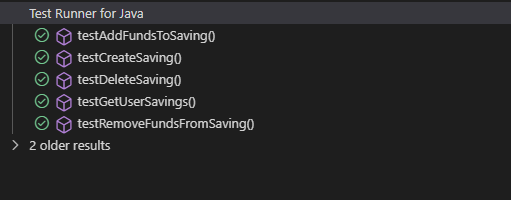
\includegraphics[width=0.9\textwidth]{images/SavingServiceTest.png}
    \caption{Test per la classe SavingService}
    \label{fig:SavingServiceTest}
\end{figure}

\begin{figure}[H]
    \centering
    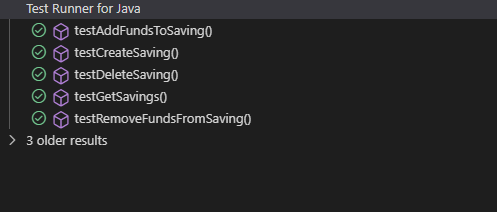
\includegraphics[width=0.9\textwidth]{images/SavingControllerTest.png}
    \caption{Test per la classe SavingController}
    \label{fig:SavingControllerTest}
\end{figure}

\begin{figure}[H]
    \centering
    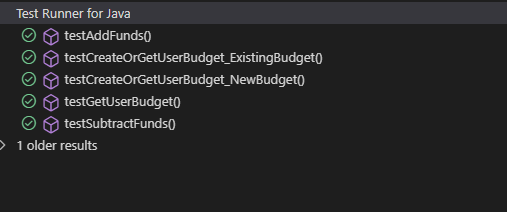
\includegraphics[width=0.9\textwidth]{images/BudgetServiceTest.png}
    \caption{Test per la classe BudgetService}
    \label{fig:BudgetServiceTest}
\end{figure}

\begin{figure}[H]
    \centering
    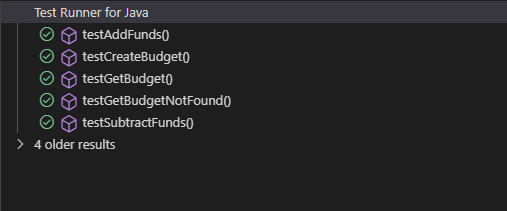
\includegraphics[width=0.9\textwidth]{images/BudgetControllerTest.png}
    \caption{Test per la classe BudgetController}
    \label{fig:BudgetControllerTest}
\end{figure}

\subsubsection{API}